\documentclass[12pt]{article}
\usepackage{moodle}
\usepackage{graphicx}

\begin{document}

\begin{quiz}{My first quiz}
\begin{numerical}[points=2]{Basic addition}
What is $8+3$?
\item 11
\end{numerical}

\begin{shortanswer}[case sensitive=true]{Panda}


\includegraphics[width = 4cm]{panda.jpg}

Is that a ?
\item Panda ?
\item[fraction=0, feedback={No, silly!}] Octopus ?
\item{fraction=0} Cat ?
\end{shortanswer}


\begin{multi}[points=3]{A first derivative}
What is the first derivative of $x^3$?
\item  $\frac{1}{4} x^4+C$
\item* $3x^2$
\item  $51$
\end{multi}

\begin{matching}[points=3.]{ExoBarsLevier}
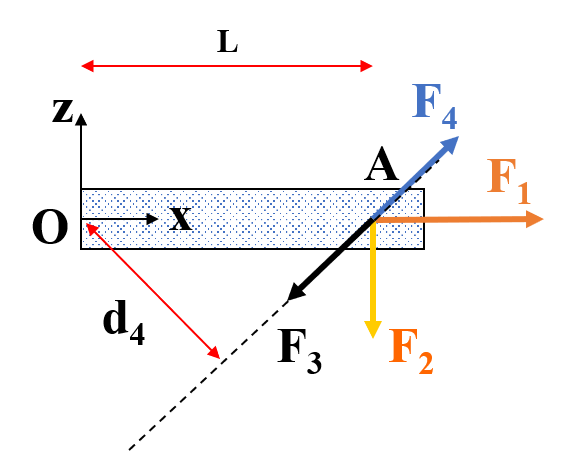
\includegraphics[width = 8cm]{BarsDeLevier}

Calculer le moment en $O$ induit par chaque force $\vec F_i$ :
\item $\vec F_1$ \answer vecteur null
\item $\vec  F_2$ \answer -F2 L
\item $\vec F_3$ \answer -F2 d4 
\item $\vec F_4$ \answer -F4 L 
\item  \answer F4 L 
\end{matching}

\end{quiz}
\end{document}